\documentclass[10pt,a4paper]{article}
\usepackage[utf8]{inputenc}
\usepackage{amsmath}
\usepackage{amsfonts}
\usepackage{amssymb}
\usepackage{graphicx}
\usepackage{rotating}

\usepackage{hyperref}
\hypersetup{
    colorlinks,
    citecolor=black,
    filecolor=black,
    linkcolor=black,
    urlcolor=black
}

\author{Ben Miller}
\title{CSE321 Project 2}
\begin{document}
\maketitle
\pagebreak
\tableofcontents
\pagebreak
\section{Specifications}
% This is the what, not the how. Should describe...
	% Inputs
	% Outputs
	% Functions
This is the documentation for a simple security system. It will lock or unlock based off of a four digit pass code, which for the purposes of this assignment will be 9407. The combination will be entered via a 4x4 matrix keypad. An LED will act as the output, lighting up depending on the validity of an input combination. Additionally, an attached LCD display will show whether the system is currently locked or unlocked.
% Will there be two LEDs? How will you differentiate a correct or incorrect response?  
\pagebreak
\section{Features}
As previously mentioned, this will be a security system that checks for an input combination of 9407. Depending on the correctness of the user's input, the system will display difference pieces of information.\\~\\
The system has four states it will ultimately check for.
\begin{itemize}
	\item An incorrect input with a locked system.
	\item An incorrect input with an unlocked system.
	\item A correct input with a locked system.
	\item A correct input with an unlocked system.
\end{itemize}
There is also a fifth state which will reset the current input; this will be described in further detail below. \\~\\
Below is how the system would react when presented with one of the above scenarios.
\begin{enumerate}
	\item An incorrect input with a locked system.
	\begin{itemize}
		\item Nothing happens, with the system remaining locked. The LCD will still display a locked mode and the LED will inform the user an incorrect input was provided. This will be done by a flashing LED.
	\end{itemize}
	\item An incorrect input with an unlocked system. 
	\begin{itemize}
		\item The system will lock. This will allow easy locking of the system by the user; they can simply input a random series of numbers. The LCD will change its display from unlocked to locked, and the LED will inform the user that an incorrect input was provided.
	\end{itemize}
	\item A correct input with a locked system.
	\begin{itemize}
		\item Of course, should a correct input be provided to an already locked system, the system will unlock. The LCD will change from locked to unlocked, and the LED will indicate a correct input. This will be shown by a steady LED.
	\end{itemize}
	\item A correct input with an unlocked system.
	\begin{itemize}
		\item Similarly to the first state, should a correct input be given to an unlocked system nothing will happen. The system will remain unlocked, with the LCD maintaining its display and the LED informing the user of a correct input.
	\end{itemize}
\end{enumerate}
\pagebreak
It was described above that there was a fifth state that will act as a ``password reset.'' This is true, and will be recognized by the system by a reserved input: 0000. This means that the system has two reserved combinations: the password itself, 9407, and the password reset key, 0000. Should at any moment four consecutive ``zeroes'' be inputted, the system will clear its memory. The LED will \textit{not} flash, and the LCD will \textit{not} change its display. This can occur at any point, regardless of how many values had previously been sent (i.e. 9-0-0-0-0 resets the memory as does 9-4-7-0-0-0-0).\\~\\
Lastly, the system can, provided power, run indefinitely. While the LED itself will not endlessly remain lit up (it will remain lit for approximately 10 seconds), the LCD display \textit{will} remain on and functional until the power source is removed.
\pagebreak
\section{Applications}
While the applications of such a simplistic security system are admittedly limited, there are some realistic applications that can be considered. A simple system such as this one can be used for minimalistic security clearance at public facilities (e.g. a supermarket). \\~\\
Given the uncomplicated implementation of the design, it can additionally be expanded upon quite easily. Changing the four-digit pass-code to an eight-digit one would be relatively straightforward, and more advanced hardware could allow for more than just the five previously described states. More advanced hardware, such as a better LCD display in conjunction with a more powerful central system, could allow multiple passwords and users to be associated with them. \\~\\
In summary, in its current state the industrial and retail applications of such a system are too limited to be of practical use; it can be brute forced due to its lack of a input cool-down, ignoring the abundantly obvious fact that such rudimentary hardware could simply be ignored. However, this simplicity is arguably an advantage, allowing for a large amount of room for expansion and improvement.
\pagebreak
\section{Block Diagram}
To be added. Currently waiting on a Piazza post.
\pagebreak
\section{Functionality Diagram}
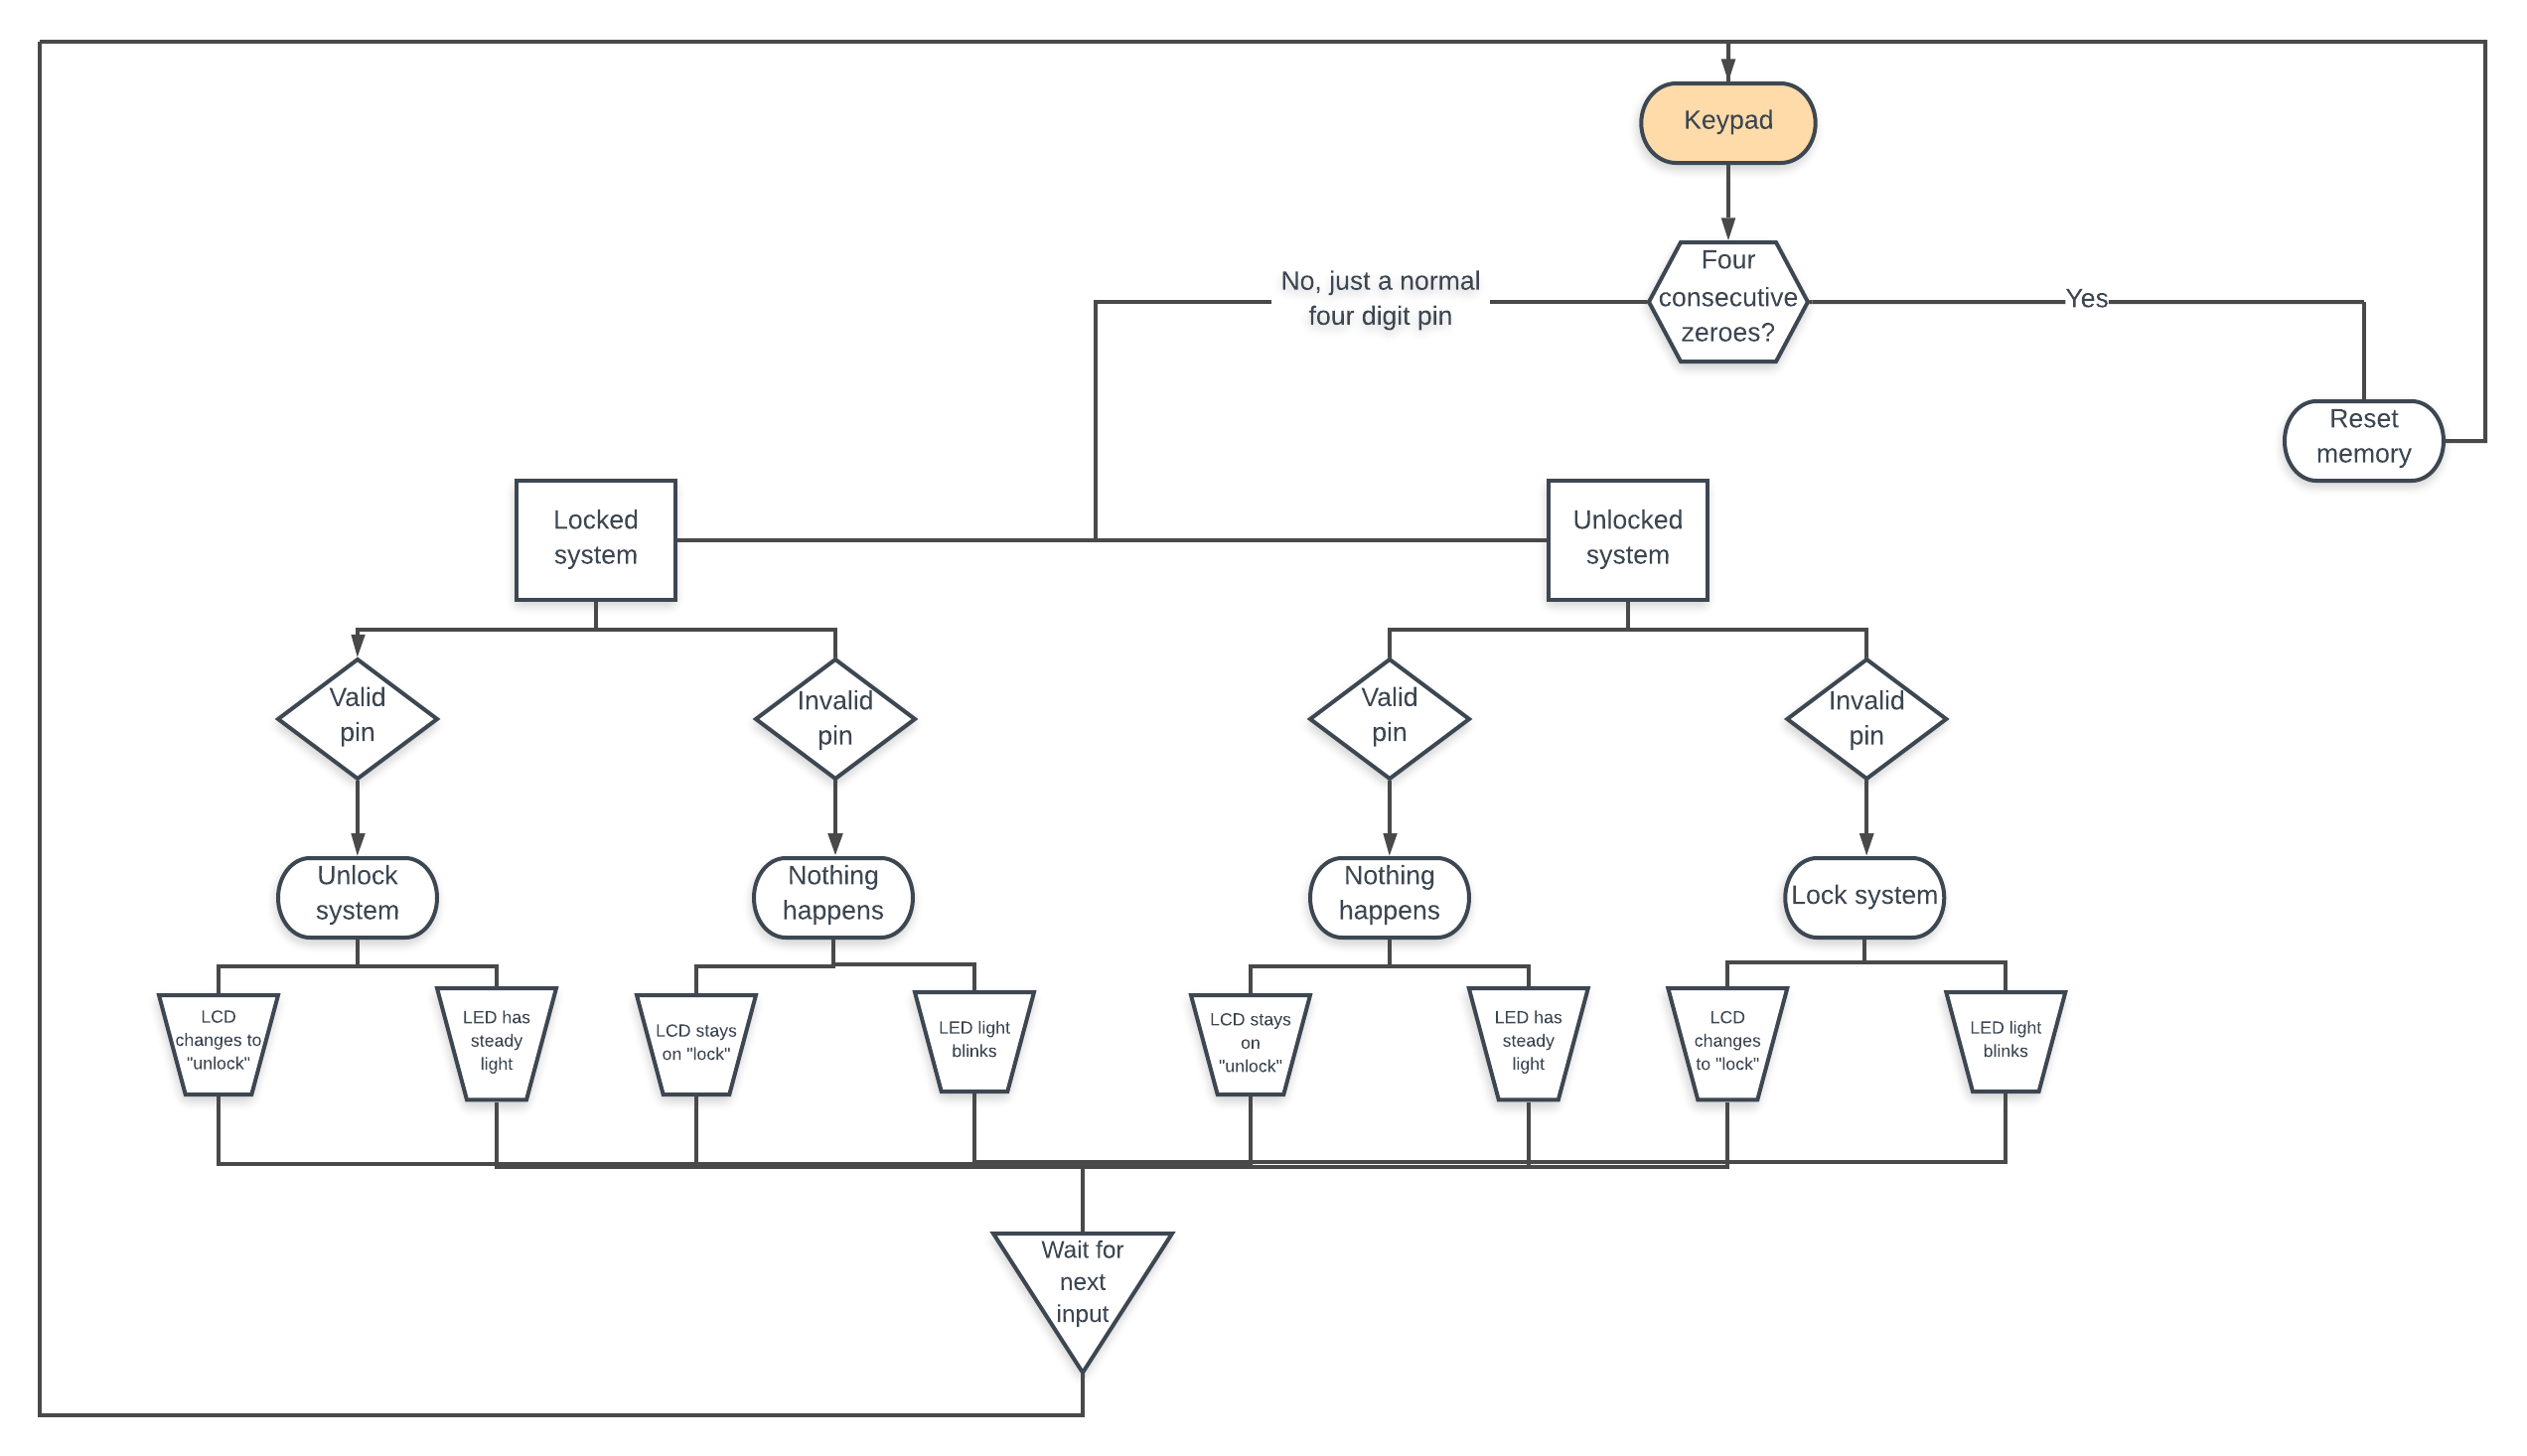
\includegraphics[width=\linewidth]{Flowchart}\\
\href{https://i.imgur.com/97heoRu.png}{\underline{Click here}} for a zoom-in-able imgur version of this image.
\pagebreak
\section{Bill of Materials}
\begin{itemize}
	\item (An unspecified amount of) LEDs
	\item A Grove 16x2 LCD display
	\item A breadboard with jumper cables and wires
	\item A Nucleo-L4R5ZI
	\item A USB A to Micro-USB B cable
	\item Resistors
	\item A 4x4 matrix array keypad
	\item Access to a desktop computer (software being used: \LaTeX and MBed Studio)
% Maybe change this? I dunno, it seems kind of barebones. It genuinely *is* all I can think of though.
\end{itemize}
\pagebreak
\section{Schematic Diagram}
To be added. Currently waiting on a Piazza post.
\pagebreak
\section{Test Plan}
To be added. 
\end{document}